\renewcommand{\theequation}{\theenumi}
\renewcommand{\thefigure}{\theenumi}
\renewcommand{\thetable}{\theenumi}
\begin{enumerate}[label=\thesection.\arabic*.,ref=\thesection.\theenumi]
\numberwithin{equation}{enumi}
\numberwithin{figure}{enumi}
\numberwithin{table}{enumi}

\item Let $\vec{A}$ be a real symmetric matrix and  $\vec{B}=\vec{I}+i\vec{A}$, where $i^2=-1$. Then choose the correct option.
\begin{enumerate}
	\item  $\vec{B}$ is invertible if and only if $\vec{A}$ is invertible.
	\item All Eigenvalues of $\vec{B}$ are necessarily real.
	\item $\vec{B}-\vec{I}$ is necessarily invertible.
	\item $\vec{B}$ is necessarily invertible.
\end{enumerate}
%
\solution
See Table \ref{eq:solutions/2017/dec/29/table:1}.

\onecolumn
\begin{longtable}{|l|l|}
\hline
\multirow{3}{*}{} & \\
Statement 1. &$\vec{B}$ is invertible if and only if $\vec{A}$ is  invertible.\\
\hline
& \\
False statement& Matrix $\vec{B}$ is invertible even if $\vec{A}$ is non invertible.\\
\hline
Example:&Consider a matrix \\&\parbox{12cm}{\begin{align}
 \vec{A}=\myvec{
1 &0 \\
0&0}\label{eq:solutions/2017/dec/29/eq1}\end{align}}\\& a real non invertible,symmetric matrix.\\&\parbox{12cm}{\begin{align}
&\implies\vec{B}=\myvec{1 & 0\\ 0 & 1}+i\myvec{1 & 0\\ 0 & 0}=\myvec{1+i & 0\\ 0 & 1  }\label{eq:solutions/2017/dec/29/eq2}\end{align}}\\ 

&is invertible even if $\vec{A}$ is non invertible.\\
\hline

%\pagebreak
%\hline
\multirow{3}{*}&\\
Statement 2. & All Eigenvalues of $\vec{B}$ are necessarily real.\\
\hline
&\\
False statement& Matrix $\vec{B}$ can have complex Eigenvalues.\\
\hline
Proof  :& Eigen values of $\vec{B}$ = Eigen values of     
($\vec{I}$) + i (Eigen values of $\vec{A}$).
\\&Clearly from \eqref{eq:solutions/2017/dec/29/eq2} above Eigen values of $\vec{B}$ are  $1$ and $1+i$   respectively.\\
& Hence $\vec{B}$ can also have complex Eigen value.\\
     \hline
\multirow{3}{*} & \\ 
Statement 3.  & $\vec{B}-\vec{I}$ is necessarily invertible.\\
\hline
&\\
False statement& $\vec{B}-\vec{I}=i\vec{A}$ will be invertible if $\vec{A}$, is invertible.\\\hline
&\\
Proof: & We have $\vec{B}-\vec{I}=i\vec{A}$\\
&$\implies \vec{B-I}=i\vec{A}=\myvec{i & 0\\ 0 & 0}$,from \eqref{eq:solutions/2017/dec/29/eq1}\\
 &Hence $\vec{B-I}$ is not invertible,unless $\vec{A}$ is invertible. \\
\hline
\multirow{3}{*}&\\
Statement 4. & $\vec{B}$ is necessarily invertible.\\
\hline
& \\
Correct Statement:& Matrix $\vec{B}$ has non zero Eigen values corresponding to Eigenvector $X$ .\\
\hline
Proof:& Let $X$ be an Eigen vector of $\vec{A}$ corresponding to Eigen value $\lambda$\\
&\\
&also,$\lambda\epsilon \mathbb{R}$\\
&\\
&$\implies$ $\vec{A}$$X$=$\lambda X $\\
&\\
&$\therefore$ $\vec{B}$$X=(\vec{I}+i\vec{A})X$= $\vec{I}$$X$+i$\vec{A}$$X$= $X$+$i\lambda$$X$\\
&\\
& $\implies$$\vec{B}$$X$ = $(1+i\lambda)$$X$\\
& Therefore, $1+i\lambda$ is an Eigen value of $\vec{B}$,\\
& corresponding to Eigen vector $X$,which are non zero.\\
& Hence, $\vec{B}$ is necessarily invertible.\\
\hline
\caption{Solution summary}
\label{eq:solutions/2017/dec/29/table:1}
\end{longtable}





\twocolumn
\item Let $\vec{A}=\myvec{0&1\\-1&1}$. Then the smallest positive integer n such that $\vec{A}^n=\vec{I}$ is
%
\\
\solution
{\em Property of eigen values of A: }
%\label{eq:solutions/2017/dec/30/section:prop}
Let $\vec{A}$ be an arbitary $n\times n$ matrix of complex numbers with eigen values $\lambda_1,\lambda_2,\hdots,\lambda_n$. Then  the eigen values of k\textsuperscript{th} power of $\vec{A}$, that is the eigen values of $\vec{A}^k$, for any positive integer k are $\lambda_1^k,\lambda_2^k,\hdots,\lambda_n^k$.
Let us calculate the eigen values of $\vec{A}$.
\begin{align}
\vec{A}=\myvec{0&1\\-1&1}\\
\det({\vec{A}-\lambda\vec{I}})=0\\
\mydet{-\lambda&1\\-1&1-\lambda}=0\\
-\lambda(1-\lambda)+1=0\\
\lambda^2-\lambda+1=0\\
\implies \lambda=\frac{-1\pm \sqrt{3}i}{2}
\end{align}
From the above property,
%\ref{eq:solutions/2017/dec/30/section:prop}, 
the eigen values of $\vec{A}^n$ are $\lambda^n$. Also as it is given that $\vec{A}^n=\vec{I}$, 
\begin{align}
\implies \lambda^n=1\\
\implies \brak{\frac{-1\pm \sqrt{3}i}{2}}^n=1
\end{align}
Clearly $n\ne 1$. For $n=2$,
\begin{align}
\brak{\frac{-1\pm \sqrt{3}i}{2}}^2=\frac{-1\mp \sqrt{3}i}{2}
\end{align}
For $n=4$,
\begin{align}
\brak{\frac{-1\pm \sqrt{3}i}{2}}^4=\frac{-1\pm \sqrt{3}i}{2}
\end{align}
For $n=6$,
\begin{align}
\brak{\frac{-1\pm \sqrt{3}i}{2}}^6=1
\end{align}
Hence $n=6$ is the smallest positive integer.

%
\item Let $\vec{A} = \myvec{1&-1&1\\1&1&1\\2&3&\alpha}$ and $\vec{b}= \myvec{1\\3\\\beta}$. Then the system $\vec{AX}=\vec{b}$ over the real numbers has\\
\begin{enumerate}
    \item No solution when $\beta \ne 7$
    \item Infinite number of solutions when $\alpha \ne 2$
    \item Infinite number of solutions when $\alpha = 2$ and $\beta \ne 7$
    \item A unique solution if $\alpha \ne 2$
\end{enumerate}
%
\solution
First we derive the Row Reduced Echelon Form (RREF) of the augmented matrix of the system $\vec{AX} = \vec{b}$ as follows,
\begin{align}
\myvec{1&-1&1&1\\1&1&1&3\\2&3&\alpha&\beta}&\xleftrightarrow[R_3=R_3-2R_1]{R_2=R_2-R_1}\myvec{1&-1&1&1\\0&2&0&2\\0&5&\alpha-2&\beta-2}\\
&\xleftrightarrow{R_2=\frac{1}{2}R_2}\myvec{1&-1&1&1\\0&1&0&1\\0&5&\alpha-2&\beta-2}\\
&\xleftrightarrow{R_1=R_1+R_2}\myvec{1&0&1&2\\0&1&0&1\\0&5&\alpha-2&\beta-2}\\
&\xleftrightarrow{R_3=R_3-5R_2}\myvec{1&0&1&2\\0&1&0&1\\0&0&\alpha-2&\beta-7}\label{eq:solutions/2017/dec/31/eq}
\end{align}
From the RREF of the augmented matrix of the system $\vec{AX} = \vec{b}$ in \eqref{eq:solutions/2017/dec/31/eq} we make the following observations for different values of $\alpha$ and $\beta$ in Table \ref{eq:solutions/2017/dec/31/table}.
, 
\begin{table}[ht!]
\begin{center}
\begin{tabular}{|c|c|}
\hline
Values & Observations\\
\hline
& Then the existence of solution and \\
$\beta \ne 7$ & the number of solutions will entirely \\
& depend on  value of $\alpha$\\
\hline
& Then RREF in \eqref{eq:solutions/2017/dec/31/eq} will contain \\
$\alpha = 2$ & Zero Row in $R_3$. Moreover solvability\\
$\beta \ne 7$ & condition will not satisfy. \\
& $\implies$ system will have Zero solutions\\
\hline
& RREF in \eqref{eq:solutions/2017/dec/31/eq} will have all pivots\\
$\alpha \ne$ 2 & $\implies$ RREF in \eqref{eq:solutions/2017/dec/31/eq} will be fullrank\\
& $\implies$ $\vec{AX}=\vec{b}$ have unique solution.\\
\hline
\end{tabular}
\end{center}
\caption{}
\label{eq:solutions/2017/dec/31/table}
\end{table}\\
Hence, if $\alpha \ne 2$ then the system $\vec{AX} = \vec{b}$ has unique solution.

%
\item Consider a Markov chain $\{X_n \: | \: n \geq 0\}$ with state space $\{1,2,3\}$ and transition matrix
\begin{align}
    \vec{P} = \myvec{0 & \frac{1}{2} & \frac{1}{2} \\
    \frac{1}{2} & 0 & \frac{1}{2} \\
    \frac{1}{2} & \frac{1}{2} & 0} \nonumber
\end{align}
Then, $P(X_3 = 1 \: | \: X_0 = 1)$ equals
%
\\
\solution
%
%
The three step transitional probabilities are given as,
\begin{align}
    P(X_3 = j \: | \: X_0 = i) = P(X_{n+3} = j \: | \: X_n = i) = \nonumber \\
    (\vec{P}^3)_{ij} \: for \: any \: n
\end{align}

\begin{align} \label{eq:solutions/2017/dec/51/eq:3_1}
    \vec{P}^3 = \myvec{0 & \frac{1}{2} & \frac{1}{2} \\
    \frac{1}{2} & 0 & \frac{1}{2} \\
    \frac{1}{2} & \frac{1}{2} & 0}^3 = 
    \myvec{\frac{1}{4} & \frac{3}{8} & \frac{3}{8} \\
    \frac{3}{8} & \frac{1}{4} & \frac{3}{8} \\
    \frac{3}{8} & \frac{3}{8} & \frac{1}{4}}
\end{align}
From \eqref{eq:solutions/2017/dec/51/eq:3_1},
\begin{align}
    P(X_3 = 1 \: | \: X_0 = 1) = (\vec{P}^3)_{11} = \frac{1}{4}
\end{align}

%
%\item 
%
%\\
%\solution
%See Table \ref{eq:solutions/2017/dec/75/table:1}.

\onecolumn
\begin{longtable}{|l|l|}
\hline
\multirow{3}{*}{} & \\
Statement 1. & A  is necessarily diagonalizable over $\vec{R}$\\
\hline
& \\
False statement& Matrix A is diagonalizable if and only if there is a basis of $\vec{R}^3 $consisting of\\
& eigenvectors of A.\\
Example:&Consider a matrix\\&\parbox{12cm}{\begin{align}
 \myvec{
1 &1 &0\\
0&1&1\\
0&0&4}\end{align}}\\
&Eigen values are:\\
&\parbox{12cm}{\begin{align}
 \myvec{
1 -\lambda &1 &0\\
0&1-\lambda&1\\
0&0&4-\lambda}=0.
\implies\lambda_1=1,\lambda_2=4\end{align}}\\
&\parbox{12cm}{\begin{align}
  \lambda_1=1\text { has eigen vector}
 \myvec{1\\0\\0} \text{and} 
  \lambda_2=4 \text{ has eigen vector}
\myvec{1\\3\\9}
\end{align}}\\
 & We have found only two linearly independent eigenvectors for A,not diagonalisable
\\
\hline
\multirow{3}{*}&\\
Statement 2. & If A has distinct real  eigen values
 than  it is diagonalizable over$\vec{R}$\\
\hline
&\\
True statement& Distinct real eigenvalues implies linearly independent eigenvectors .\\
& and if a matrix has n linearly independent vectors than it is  diagonalizable.\\
\hline
Proof  1:& \textbf{Distinct eigen values implies linearly independent vectors that spans entire space.}\\&Consider 2 eigen vectors $\vec{v}$,$\vec{w}$  with eigen values $\lambda$,$\mu$ respectively.\\
& such that $\lambda\neq\mu$\\
 &\parbox{12cm}{\begin{align}
    \alpha(\vec{v})+\beta(\vec{w})=0\label{eq:solutions/2017/dec/75/eq2}\\
     \alpha A(\vec{v})+\beta A(\vec{w})=0\\
     \alpha \lambda\vec{v}+\beta\mu\vec{w}=0\label{eq:solutions/2017/dec/75/eq3}
     \end{align}}\\
     & Multiplying $\eqref{eq:solutions/2017/dec/75/eq2}$with -$\lambda$ and subtracting from $\eqref{eq:solutions/2017/dec/75/eq3}$ we have,\\
   & \parbox{12cm}{\begin{align}  
  \beta(\mu-\lambda)\vec{w}=0 \label{eq:solutions/2017/dec/75/eq1}
  \end{align}}\\
  & eigen values are distinct $(\mu-\lambda)\neq 0$ .
  From equation$\eqref{eq:solutions/2017/dec/75/eq1}$ we have, $\beta=0$\\
  & substituting $\beta=0$ in  equation $\eqref{eq:solutions/2017/dec/75/eq2}$we have,$\alpha=0$.As, $\vec{v}\neq 0$\\
  & \textbf{which proves that vectors are linearly independent}.\\
  
  Proof 2:
 & \textbf{If a matrix has n linearly independent vectors than it is diagonalizable}\\
 & If\myvec{
\vec{p_1} &\vec{p_2}&\cdots&\vec{p_n} 
}are n independent eigen vectors then,
 $A\vec{p_1}=\lambda \vec{p_1},\cdots ,A\vec{p_n}=\lambda \vec{p_n}$\\
&\parbox{12cm}{\begin{align}{D}=\myvec{\lambda_1&0&\cdots&0\\
0&\lambda_2&\cdots&0\\
\vdots&\vdots&\vdots&\vdots\\
0&0&\cdots&\lambda_n}
 \and{P}=\myvec{
\vec{P_1}& \vec{P_2}&\cdots& \vec{P_n}
}\end{align}}\\
& Now, $A\vec{P_i}=\lambda_i\vec{P_i}$ $\implies$ ${A}{P}={P}{D}$\\
& so,${P^{-1}}{AP}={D}$ is a diagonal matrix.\\
    \hline
\multirow{3}{*} & \\ 
Statement 3.  & If A has distinct real  eigen values
 than  it is diagonalizable over$\vec{C}$\\
\hline
&\\
True statement& If A is an $N \times N$ complex matrix with n distinct eigenvalues, then any set of\\
& n corresponding eigenvectors form a basis for $\vec{C}^n$\\ .
&\\
Proof: &It is sufficient to prove that the set of eigenvectors is linearly independent \\
&which is proved in statement 2.\\
 Example:&\parbox{12cm}{\begin{align}A=\myvec{
4& 0 &-2\\
2& 5 &4\\
0& 0 &5
}\end{align}}\\
& Eigen values of A are:\\
& \parbox{12cm}{\begin{align}\lambda_1=2,\lambda_2=3 , \lambda_3=6\end{align}}\\
\hline
& Eigen vectors are:\\&\parbox{12cm}{\begin{align}x_1=\myvec{
-1\\1\\0
},
x_ 2=\myvec{
1\\1\\1
},
x_3=\myvec{
-1\\ - 1\\ 2
}\end{align}}
\\
 & Matrix A is diagonalizable because there is a basis of $\vec{C}^3 $consisting of\\
& eigenvectors of A.\\
\hline
\multirow{3}{*}&\\
Statement 4. & If all eigen values are non zero than it is diagonalizable over $\vec{C}$\\
\hline
& \\
False Statement:& Matrix would be diagonalizable if and only if it has linearly independent eigenvectors .\\
\hline
Example:&Consider a matrix\\&\parbox{12cm}{\begin{align}
 \myvec{
1 &1 &0\\
0&1&1\\
0&0&4}\end{align}}\\
&Eigen values are:\\
&\parbox{12cm}{\begin{align}
 \myvec{
1 -\lambda &1 &0\\
0&1-\lambda&1\\
0&0&4-\lambda}=0.
\implies\lambda_1=1,\lambda_2=4\neq 0\end{align}}\\
&\parbox{12cm}{\begin{align}
  \lambda_1=1\text { has eigen vector}
 \myvec{1\\0\\0} \text{and} 
  \lambda_2=4 \text{ has eigen vector}
\myvec{1\\3\\9}
\end{align}}\\
 & We have found only two linearly independent eigenvectors for A,not diagonalisable.\\
 &\\
\hline
\caption{Solution summary}
\label{eq:solutions/2017/dec/75/table:1}
\end{longtable}

   


\item 	Let $\vec{A}$ be an $m\times n$ matrix with rank $r$. If the linear system $\vec{A}\vec{X} = \vec{b}$ has a solution for each $\vec{b} \in \mathbf{R}^{m}$, then
	\begin{enumerate}
		\item $m=r$
		\item the column space of $\vec{A}$ is a proper subspace of $\mathbf{R}^{m}$ 
		\item the null space of $\vec{A}$ is a non-trivial subspace of $\mathbf{R}^{n}$ whenever $m=n$
		\item $m\geq n$ implies $m=n$
	\end{enumerate}
%
\solution
	{\em Theorem}
	
	\begin{theorem}\label{eq:solutions/2017/dec/72/thm1}
		Consider the $m\times n$ system Ax = b, with either b $\neq$ 0 or b = 0. We distinguish the following cases:
		\begin{enumerate}
			\item $\textbf{Unique Solution}$: If rank[A,b] = rank(A) = n $\leq$ m, then and only then the system has a unique solution. In this case, indeed as many as $m-n$ equations are redundant. And the solution $\vec{X} = {\vec{A}^{-1}\vec{b}}$. This is called as $\textbf{Exactly Determined}$.
			\item $\textbf{No Solution}$: If rank[A,b] $>$ rank(A) which necessarily implies $\Vec{b} \neq 0$ and m $>$ rank(A), then and only then the system has no solution. This is called as $\textbf{Overdetermined}$.
		\end{enumerate}
	\end{theorem}
See Table \ref{eq:solutions/2017/dec/72/table}
%	
		If the columns of an $m\times n$ matrix $\Vec{A}$ span $\vec{R}^{m}$ then the equation $\vec{A}\vec{x}=\vec{b}$ is consistent for each $\Vec{b}$ in $\vec{R}^{m}$. \\ \\
	The $\textbf{null space}$ of $\vec{A}$ is defined to be 
	
	\begin{align}\label{eq:solutions/2017/dec/72/eq1}
		Null(\vec{A}) = \{ \vec{x} \in \mathbf{R}^{n} \, \vert \, \vec{A}\vec{x} = 0 \}
	\end{align}
%	
	%	Let $\vec{A}$ be given as
	
	\begin{align} \label{eq:solutions/2017/dec/72/eq2}
		\vec{A} = \myvec{-3&-2&4 \\ 14&8&-18 \\ 4&2&-4}
	\end{align}
	
	Reduced Row Echelon form is
	
	\begin{align}
		RREF\left(\vec{A}\right) = \myvec{1&0&0 \\ 0&1&0 \\ 0&0&1}
	\end{align}
	$\therefore$ the only possible nullspace of the matrix $\vec{A}$ is $\myvec{0\\0\\0}$.\\
	
	
	Let $\vec{B}$ be given as
	
	\begin{align} \label{eq:solutions/2017/dec/72/eq3}
		\vec{B} = \myvec{-3&-2&4 \\ 14&8&-18 \\ 4&2&-4 \\ 28&16&-36 \\ 8&4&-8}
	\end{align}
	
	Reduced Row Echelon form is
	
	\begin{align}
		RREF\left(\vec{B}\right) = \myvec{1&0&0 \\ 0&1&0 \\ 0&0&1 \\ 0&0&0 \\ 0&0&0}
	\end{align}
	$\therefore$ the rank of matrix $\vec{B} = 3$.
	
	\begin{table*}[!ht]
%\centering
		\begin{tabular}{|l|l|}
			\hline
			Options & Observations\\
			\hline
			& \\
			& The rank of any matrix $\vec{A}$ is the dimension of its column space. When  \\
			$m = r$&  the number of rows ($m$) is equal to the rank ($r$) of the matrix, then \\
			&  their linear combination gives us span of $\vec{R}^{m}$.\\
			& \\
			& $\therefore$ This statement is $\textbf{True}$. \\
			& \\
			\hline 
			& \\
			& Any subspace of a vector space $\vec{V}$ other than $\vec{V}$ itself is considered a \\
			the column & proper subspace of $\vec{V}$. Which means that linear combination of $\vec{A}$\\
			space of $\vec{A}$ & will span less than $m$. That will make the resultant\\
			is a proper & $\vec{b}$ span strictly less than $m$.\\ 
			subspace of & But it is given that $\vec{b} \in \mathbf{R}^{m}$, which is contradicting.\\  
			$\mathbf{R}^{m}$ & \\
			& $\therefore$ This statement is $\textbf{False}$. \\
			& \\
			\hline
			& \\
			the null & From $\eqref{eq:solutions/2017/dec/72/eq2}$ we see that even when $m = n$ then also we are getting a\\ 
			space of $\vec{A}$ & trivial nullspace. \\
			is a non-trivial& \\
			subsapce of $\mathbf{R}^{n}$& \\
			whenever $m=n$& $\therefore$ This statement is $\textbf{False}$. \\
			& \\
			\hline
			& \\
			& It is given that the number of rows are greater than the column, and it \\
			$m \geq n$ & is given that there exists a solution. If we refer to theorem $\eqref{eq:solutions/2017/dec/72/thm1}$ we \\
			implies & see that the corresponding system will be $\textbf{Exactly Determined}$ system. \\
			$m=n$ & \\
			& As an example, it will look like $\eqref{eq:solutions/2017/dec/72/eq3}$.\\
			& \\
			& $\therefore$ This statement is $\textbf{True}$. \\
			& \\
			\hline
		\end{tabular}
\caption{Solution}
\label{eq:solutions/2017/dec/72/table}
	\end{table*}
	

\item Let $\vec{M}$ =$\cbrak{\myvec{a&b\\c&d} : a,b,c,d \in \mathbb{Z} \text{ and eigen values of} \vec{A} \in \mathbb{Q}}$ \label{main}
\begin{enumerate}
    \item $\vec{M}$ is empty
    \item $\vec{M}$ =\cbrak{\myvec{a&b\\c&d} : a,b,c,d \in \mathbb{Z}}
    \item If $\vec{A}$ $\in$ $\vec{M}$ then the eigen values of $\vec{A}$ $\in$ $\mathbb{Z}$
    \item If $\vec{A}$,$\vec{B}$ $\in$ $\vec{M}$ such that $\vec{A} \vec{B}$=$\vec{I}$ then $\mydet{\vec{A}}$ $\in$ \{+1,-1\}
\end{enumerate}
%
\solution
See Table \ref{table:2017/dec/74/}.
\onecolumn
	\begin{longtable}{|l|l|}
	\hline
	\multirow{3}{*}{$\vec{M}$ is empty} & \\
	& Consider $\vec{A}$=$\vec{I}$=\myvec{1&0\\0&1}.The elements of $\vec{A}$ $\in$ $\mathbb{Z}$ and it's eigen values 1 $\in$ $\mathbb{Q}$.\\
	&So, $\vec{M}$ is not empty. \\
	& \\
	\hline
	\multirow{3}{*}{$\vec{M}$ =\cbrak{\myvec{a&b\\c&d} : a,b,c,d \in \mathbb{Z}}} & \\
	& Let $\vec{A}$=\myvec{0&-1\\1&0} where elements of $\vec{A}$ $\in$ $\mathbb{Z}$.The characteristic equation can be \\ 
	& written as :\\
	& \\
	& \qquad \qquad \qquad$ \lambda^2+1 = 0 \implies \lambda = \pm i$ \\
	& \\
	& We see that $\lambda$ $\in$ $\mathbb{C}$ which is contradicting the main definition of $\vec{M}$ .So,this \\
	& is not correct. \\
	& \\
	\hline
	\multirow{3}{*}{Eigen values of $\vec{A}$ $\in$ $\mathbb{Z}$} & \\
	& Given ,$\vec{A}$ $\in$ $\vec{M}$.Let $\lambda_1$,$\lambda_2$ be the eigen values of $\vec{A}$.The characteristic polynomial \\ 
	&can be written as:\\
	& \\
	& \qquad \qquad \qquad$ \lambda^2-tr\brak{\vec{A}}\lambda +\det{\vec{A}}= 0 $ where $tr\brak{\vec{A}}=\lambda_1+\lambda_2,\det{\vec{A}}=\lambda_1\lambda_2$\\
	& \\
	& Given the eigen values $\lambda\_1$,$\lambda\_2$  $\in$ $\mathbb{Q}$,For this to be possible the discriminant \\
	& of above equation should $\in$ $\mathbb{Z}$\\
	& \qquad \qquad \qquad$\sqrt{(\lambda_1+\lambda_2)^2-4\lambda_1\lambda_2} \in \mathbb{Z}$ \\
	& \qquad \qquad$\implies \sqrt{(\lambda_1-\lambda_2)^2} \in \mathbb{Z}$ \\
	& \qquad \qquad$\implies \lambda_1-\lambda_2 \in \mathbb{Z}$ 
	This is possible when both $\lambda_1$,$\lambda_2$ $\in$ $\mathbb{Z}$.\\
	& \\
	\hline
	\multirow{3}{*}{If $\vec{A} \vec{B}$=$\vec{I}$ then $\mydet{\vec{A}}$ $\in$ \{+1,-1\}} 
	& \\
	& As $\vec{A}$,$\vec{B}$ $\in$ $\vec{M}$,$\implies$ $\mydet{\vec{A}}$,$\mydet{\vec{B}}$ $\in$ $\mathbb{Z}$ \\
	& Given $\vec{A}\vec{B}$=$\vec{I}$ $\implies$ $\mydet{\vec{A}}\mydet{\vec{B}}$=1\\
	& This is possible only when $\mydet{\vec{A}}$=$\mydet{\vec{B}}$= $\pm$ 1\\
	& \\
	\hline
	\multirow{3}{*}{Conclusion} & \\
	& options 3) and 4) are correct.\\
    & \\
	\hline
\caption{Solution}
\label{table:2017/dec/74/}
    \end{longtable}

%
\item Let A be a $3\times 3$  matrix  with real entries.Identify  the correct statements.
\begin{enumerate}

\item A  is necessarily diagonalizable over $\vec{R}$

\item If A has distinct real  eigen values than  it is diagonalizable over$\vec{R}$

\item If A has distinct eigen values than  it is diagonalizable over $\vec{C}$

\item If all eigen values are non zero than it is diagonalizable over $\vec{C}$
\end{enumerate}
%
\solution
See Table \ref{eq:solutions/2017/dec/75/table:1}.

\onecolumn
\begin{longtable}{|l|l|}
\hline
\multirow{3}{*}{} & \\
Statement 1. & A  is necessarily diagonalizable over $\vec{R}$\\
\hline
& \\
False statement& Matrix A is diagonalizable if and only if there is a basis of $\vec{R}^3 $consisting of\\
& eigenvectors of A.\\
Example:&Consider a matrix\\&\parbox{12cm}{\begin{align}
 \myvec{
1 &1 &0\\
0&1&1\\
0&0&4}\end{align}}\\
&Eigen values are:\\
&\parbox{12cm}{\begin{align}
 \myvec{
1 -\lambda &1 &0\\
0&1-\lambda&1\\
0&0&4-\lambda}=0.
\implies\lambda_1=1,\lambda_2=4\end{align}}\\
&\parbox{12cm}{\begin{align}
  \lambda_1=1\text { has eigen vector}
 \myvec{1\\0\\0} \text{and} 
  \lambda_2=4 \text{ has eigen vector}
\myvec{1\\3\\9}
\end{align}}\\
 & We have found only two linearly independent eigenvectors for A,not diagonalisable
\\
\hline
\multirow{3}{*}&\\
Statement 2. & If A has distinct real  eigen values
 than  it is diagonalizable over$\vec{R}$\\
\hline
&\\
True statement& Distinct real eigenvalues implies linearly independent eigenvectors .\\
& and if a matrix has n linearly independent vectors than it is  diagonalizable.\\
\hline
Proof  1:& \textbf{Distinct eigen values implies linearly independent vectors that spans entire space.}\\&Consider 2 eigen vectors $\vec{v}$,$\vec{w}$  with eigen values $\lambda$,$\mu$ respectively.\\
& such that $\lambda\neq\mu$\\
 &\parbox{12cm}{\begin{align}
    \alpha(\vec{v})+\beta(\vec{w})=0\label{eq:solutions/2017/dec/75/eq2}\\
     \alpha A(\vec{v})+\beta A(\vec{w})=0\\
     \alpha \lambda\vec{v}+\beta\mu\vec{w}=0\label{eq:solutions/2017/dec/75/eq3}
     \end{align}}\\
     & Multiplying $\eqref{eq:solutions/2017/dec/75/eq2}$with -$\lambda$ and subtracting from $\eqref{eq:solutions/2017/dec/75/eq3}$ we have,\\
   & \parbox{12cm}{\begin{align}  
  \beta(\mu-\lambda)\vec{w}=0 \label{eq:solutions/2017/dec/75/eq1}
  \end{align}}\\
  & eigen values are distinct $(\mu-\lambda)\neq 0$ .
  From equation$\eqref{eq:solutions/2017/dec/75/eq1}$ we have, $\beta=0$\\
  & substituting $\beta=0$ in  equation $\eqref{eq:solutions/2017/dec/75/eq2}$we have,$\alpha=0$.As, $\vec{v}\neq 0$\\
  & \textbf{which proves that vectors are linearly independent}.\\
  
  Proof 2:
 & \textbf{If a matrix has n linearly independent vectors than it is diagonalizable}\\
 & If\myvec{
\vec{p_1} &\vec{p_2}&\cdots&\vec{p_n} 
}are n independent eigen vectors then,
 $A\vec{p_1}=\lambda \vec{p_1},\cdots ,A\vec{p_n}=\lambda \vec{p_n}$\\
&\parbox{12cm}{\begin{align}{D}=\myvec{\lambda_1&0&\cdots&0\\
0&\lambda_2&\cdots&0\\
\vdots&\vdots&\vdots&\vdots\\
0&0&\cdots&\lambda_n}
 \and{P}=\myvec{
\vec{P_1}& \vec{P_2}&\cdots& \vec{P_n}
}\end{align}}\\
& Now, $A\vec{P_i}=\lambda_i\vec{P_i}$ $\implies$ ${A}{P}={P}{D}$\\
& so,${P^{-1}}{AP}={D}$ is a diagonal matrix.\\
    \hline
\multirow{3}{*} & \\ 
Statement 3.  & If A has distinct real  eigen values
 than  it is diagonalizable over$\vec{C}$\\
\hline
&\\
True statement& If A is an $N \times N$ complex matrix with n distinct eigenvalues, then any set of\\
& n corresponding eigenvectors form a basis for $\vec{C}^n$\\ .
&\\
Proof: &It is sufficient to prove that the set of eigenvectors is linearly independent \\
&which is proved in statement 2.\\
 Example:&\parbox{12cm}{\begin{align}A=\myvec{
4& 0 &-2\\
2& 5 &4\\
0& 0 &5
}\end{align}}\\
& Eigen values of A are:\\
& \parbox{12cm}{\begin{align}\lambda_1=2,\lambda_2=3 , \lambda_3=6\end{align}}\\
\hline
& Eigen vectors are:\\&\parbox{12cm}{\begin{align}x_1=\myvec{
-1\\1\\0
},
x_ 2=\myvec{
1\\1\\1
},
x_3=\myvec{
-1\\ - 1\\ 2
}\end{align}}
\\
 & Matrix A is diagonalizable because there is a basis of $\vec{C}^3 $consisting of\\
& eigenvectors of A.\\
\hline
\multirow{3}{*}&\\
Statement 4. & If all eigen values are non zero than it is diagonalizable over $\vec{C}$\\
\hline
& \\
False Statement:& Matrix would be diagonalizable if and only if it has linearly independent eigenvectors .\\
\hline
Example:&Consider a matrix\\&\parbox{12cm}{\begin{align}
 \myvec{
1 &1 &0\\
0&1&1\\
0&0&4}\end{align}}\\
&Eigen values are:\\
&\parbox{12cm}{\begin{align}
 \myvec{
1 -\lambda &1 &0\\
0&1-\lambda&1\\
0&0&4-\lambda}=0.
\implies\lambda_1=1,\lambda_2=4\neq 0\end{align}}\\
&\parbox{12cm}{\begin{align}
  \lambda_1=1\text { has eigen vector}
 \myvec{1\\0\\0} \text{and} 
  \lambda_2=4 \text{ has eigen vector}
\myvec{1\\3\\9}
\end{align}}\\
 & We have found only two linearly independent eigenvectors for A,not diagonalisable.\\
 &\\
\hline
\caption{Solution summary}
\label{eq:solutions/2017/dec/75/table:1}
\end{longtable}

   


\twocolumn
\item Let $V$ be a vector space over $C$ of all the polynomials in a variable $X$ of degree atmost 3. Let $D:V \xrightarrow{} V$ be the linear operator given by differentiation with respect to $X$. Let $A$ be the matrix of $D$ with respect to some 
basis for $V$. Which of the following are true? \\
\begin{enumerate}
\item A is nilpotent matrix \\
\item A is diagonalizable matrix \\ 
\item the rank of A is 2 \\
\item the Jordan canonical form of A is
\begin{align}\nonumber
    \myvec{0&1&0&0\\
       0&0&1&0\\
       0&0&0&1\\
       0&0&0&0}
\end{align}
\end{enumerate}
%
\solution
See Tables \ref{eq:solutions/2017/dec/76/table0}, \ref{eq:solutions/2017/dec/76/table2} and \ref{eq:solutions/2017/dec/76/table1}


\begin{table*}[ht!]
\begin{center}
\begin{tabular}{|c|c|}
\hline
& \\
Given & $V$ be a vector space over $C$ of all the polynomials in a variable $X$ of degree atmost 3\\
& $D$ : $P_3 \xrightarrow{} P_3$ \\ 
& \\
& $D:V\xrightarrow{}V$ be the linear operator given by differentiation wrt $X$\\
& $D(P(x)) \xrightarrow{}$ $P'(x)$ \\
& \\
& $A$ be the matrix of $D$ wrt some basis for $V$ \\
& Assume basis for $V$ be $\{1,x,x^2,x^3\}$ \\
& \\
\hline
\end{tabular}
\end{center}
\caption{}
\label{eq:solutions/2017/dec/76/table0}
\end{table*}
\begin{table*}[ht!]
\begin{center}
\begin{tabular}{|c|c|}
\hline
&\\
Matrix & $D(1)$ = $0$ = $0.1+0.x+$\\
& $0.x^2+0.x^3$\\
& $D(1)$ = $\myvec{0\\0\\0\\0}$ \\
& $D(x)$ = $1$ = $1.1+0.x+$\\
& $0.x^2+0.x^3$\\
& $D(x)$ = $\myvec{1\\0\\0\\0}$ \\
& $D(x^2)$ = $2x$ = $0.1+2.x+$\\
& $0.x^2+0.x^3$\\
& $D(x^2)$ = $\myvec{0\\2\\0\\0}$ \\
& $D(x^3)$ = $3x^2$ = $0.1+0.x+$\\
& $3.x^2+0.x^3$\\
& $D(x^3)$ = $\myvec{0\\0\\3\\0}$ \\
& Matrix $A$ = $\myvec{0&1&0&0\\
                0&0&2&0\\
                0&0&0&3\\
                0&0&0&0}$\\
&\\
\hline
& \\
Inference & An $n\times n$ matrix with $\lambda$\\
& as diagonal elements, ones on the\\
& super diagonal and zeroes in all\\
& other entries is nilpotent with\\
& minimal polynomial $(A-\lambda I)^n$\\
&\\
\hline
& \\
Nilpotent & $A$ = $\myvec{0&1&0&0\\
                0&0&2&0\\
                0&0&0&3\\
                0&0&0&0}$\\
& \\
& All eigen values of matrix $A$\\
& is $0$\\
& Thus, above matrix is \\
& nilpotent matrix \\
& Thus, above statement \\
& is true\\
& \\
\hline
\end{tabular}
\end{center}
\caption{}
\label{eq:solutions/2017/dec/76/table2}
\end{table*}
\begin{table*}[ht!]
\begin{center}
\begin{tabular}{|c|c|}
\hline
Diagonalizable & $A$ = $\myvec{0&1&0&0\\
                0&0&2&0\\
                0&0&0&3\\
                0&0&0&0}$\\
& $Rank(A)$ + $nullity(A)$ = no of column\\
& $Rank(A)$ = 3, no of column = 4 \\
& $nullity(A)$ = 4 - 3 = 1\\
& means there exists only one\\
& linearly independent eigen vector\\
& corresponding to $0$ eigen values\\
& Thus,matrix $A$ is not Diagonalizable.\\
& Thus, above statement is false\\
& \\
\hline
& \\
Rank & $A$ = $\myvec{0&1&0&0\\
                0&0&2&0\\
                0&0&0&3\\
                0&0&0&0}$\\
& \\
& Rank of matrix $A$ is $3$\\
& Thus, above statement is false\\
& \\
\hline
& \\
Jordan CF & Assume characteristic polynomial of \\
& matrix $A$ is $c_A(x)$ \\
& $c_A(x)$ = $x^4$ \\
& Assume minimal polynomial of\\
& $A$ is $m_A(x)$\\
& $m_A(x)$ always divide $c_A(x)$ \\
& $m_A(x)$ = $\{x,x^2,x^3,x^4\}$\\
& Minimal polynomial always annihilates\\
& its matrix.Thus,we see that\\
& $m_A(A)$ = $\{A=0,A^2=0,A^3=0,A^4=0\}$\\
& But we see that neither A is zero matrix\\
& nor $A^2$ and $A^3$ equal to zero\\
& but $A^4$ is equal to zero.Thus,$x^4$\\
& is minimal polynomial.\\
& Algebraic Multiplicity = $a_M$($\lambda$ = 0) = 4\\
& Geometric Multiplicity = $g_M$($\lambda$ = 0) = \\
& $nullity(A-0I)$ = $nullity(A)$ = 1\\
& Hence, Jordan form of block size 4\\
& Using Inference, $\vec{J} = \myvec{\lambda & 1 & 0 & 0 \\ 
                        0 & \lambda & 1 & 0\\ 
                        0 & 0 & \lambda & 1\\
                        0 & 0 & 0 & \lambda }$ \\
& $\lambda$ = 0 \\ 
& $\myvec{0&1&0&0\\
       0&0&1&0\\
       0&0&0&1\\
       0&0&0&0}$\\
& which is same as given in\\
& the question. Thus,statement is true \\
& \\
\hline
\end{tabular}
\end{center}
\caption{}
\label{eq:solutions/2017/dec/76/table1}
\end{table*}

\item For every $4 \times 4$ real symmetric non-singular matrix $\vec{A}$ there 
exists a positive integer $p$ such that

    \begin{enumerate}
        \item $p\vec{I}+\vec{A}$ is positive definite
        \item $\vec{A}^p$ is positive definite
        \item $\vec{A}^{-p}$ is positive definite
        \item $\text{exp}(p\vec{A})-\vec{I}$ is positive definite
        \end{enumerate}
\solution
%
A matrix is real symmetric implies its eigen values are real and eigen vectors are orthogonal,that is its eigen value decomposition is
\begin{align}
 \vec{A}=\vec{P}\vec{D}\vec{P}^T
\end{align}
$\vec{D}$ is the diagonal matrix containing the real eigen values of $\vec{A}$\\
$\vec{P}$ has the corresponding eigen vectors
\begin{align}
    \vec{P}\vec{P}^T=\vec{P}^T\vec{P}=\vec{I}
\end{align}
A real matrix is positive definite if 
\begin{align}
    \vec{x}^T\vec{A}\vec{x}>0\\
    \implies  \vec{x}^T\lambda\vec{x}>0\\
    \implies \lambda \vec{x}^T\vec{x}>0\\
    \implies \lambda>0
\end{align}
In other words, all the eigen values of $A$ are positive
See Table \ref{eq:solutions/2017/dec/77/table:0}

Let $\vec{A}$ be
\begin{align}
    \vec{A}=\vec{P}\vec{D}\vec{P}^T\\
    \vec{D}=\myvec{\lambda_1&0&0&0\\0&\lambda_2&0&0\\0&0&\lambda_3&0\\0&0&0&\lambda_4}
\end{align}



\begin{table*}[!t]
    \centering
    \begin{tabular}{|l|l|}
    \hline

    \textbf{OPTIONS} & \textbf{DERIVATIONS}\\
    \hline
     Choice 1 & 
      \parbox{12cm}{\begin{align}
         p\vec{I}+\vec{A}=\vec{P}(p\vec{I})\vec{P}^T+\vec{P}\vec{D}\vec{P}^T\\
   = \vec{P}\vec{D}_1\vec{P}^T\\
    \vec{D}_1=\myvec{\lambda_1+p&0&0&0\\0&\lambda_2+p&0&0\\0&0&\lambda_3+p&0\\0&0&0&\lambda_4+p}
    \end{align}}\\
     & Some of the eigen values of $\vec{A}$ may be negative.\\
     & All the eigen values in $\vec{D}_1$ are positive only if \\
     & \parbox{12cm}{\begin{align}
          p>|\lambda_i|\text{  } \forall i \in [1,4]
     \end{align}}\\
      
      \hline
      Choice 2 & 
       \parbox{12cm}{\begin{align}
          \vec{A}^2=\vec{A}\vec{A}\\
    =(\vec{P}\vec{D}\vec{P}^T)(\vec{P}\vec{D}\vec{P}^T)\\
    =\vec{P}\vec{D}^2\vec{P}^T\\
    \text{Similarly, }\vec{A}^p=\vec{P}\vec{D}^p\vec{P}^T\\
    \vec{D}^p=\myvec{\lambda_1^p&0&0&0\\0&\lambda_2^p&0&0\\0&0&\lambda_3^p&0\\0&0&0&\lambda_4^p}
       \end{align}}\\
       & $\vec{A}^{p}$ is positive definite only if $p$ is even.\\
       \hline
      Choice 3& 
        \parbox{12cm}{\begin{align}
           \vec{A}^{-p}=\vec{P}\vec{D}^{-p}\vec{P}^T\\
    \vec{D}^{-p}=\myvec{\lambda_1^{-p}&0&0&0\\0&\lambda_2^{-p}&0&0\\0&0&\lambda_3^{-p}&0\\0&0&0&\lambda_4^{-p}}
       \end{align}}\\
       & $\vec{A}^{-p}$ is positive definite only if $p$ is even.\\
       \hline
      Choice 4 &
        \parbox{12cm}{\begin{align}
          \text{exp}(p\vec{A})=\sum_{k=0}^\infty \frac{(p\vec{A})^k}{k!}\\
     \implies  \text{exp}(p\vec{A})-\vec{I}=\vec{P} \text{exp}(p\vec{D})\vec{P}^T-\vec{P}\vec{I}\vec{P}^T\\
     =\vec{P}( \text{exp}(p\vec{D})-\vec{I}) \vec{P}^T\\
     \text{exp}(p\vec{D})-\vec{I}=\myvec{e^{\lambda_1}-1&0&0&0\\0&e^{\lambda_2}-1&0&0\\0&0&e^{\lambda_3}-1&0\\0&0&0&e^{\lambda_4}-1}
       \end{align}}\\
       & $\vec{A}$ is non-singular\\
        & \parbox{12cm}{\begin{align}
   \implies \forall i \in [1,4], \lambda_i\neq0\\
   e^{\lambda_i}<1
\end{align}}\\
 & So, exp$(p\vec{A})-\vec{I}$ is not positive definite.\\
       \hline
    \end{tabular}
    \caption{Solution}
\label{eq:solutions/2017/dec/77/table:0}
\end{table*}
 From the table,the choices would be option 1,2,3





\item Let $\vec{A}$ be an $m \times n$ matrix of rank $m$ with $n>m$. If for some non-zero real number $\alpha$, we have $\vec{x^TAA^Tx} = \alpha\vec{x^Tx}$, for all $x \in \vec{R^m}$, then $\vec{A^TA}$ has,
\begin{enumerate}

\item  exactly two distinct eigenvalues.

\item  0 as an eigenvalue with multiplicity $n-m$.

\item  $\alpha$ as a non-zero eigenvalue.

\item  exactly two non-zero distinct eigenvalues.
\end{enumerate}
%
\solution
Refer Table \ref{eq:solutions/2017/dec/78/table:1}.


\begin{table*}[ht!]
\begin{center}
\resizebox{\columnwidth}{!}
{
\begin{tabular}{|l|l|}
\hline
\textbf{Given} & \textbf{Derivation} \\[0.5ex]
\hline
\text{Given} & 
\text{$\vec{A}$ is a $m \times n$ matrix of rank $m$ with $n>m$}. \\
& A non-zero real number $\alpha$.\\
& To find eigenvalues of $\vec{A^TA}$.
\\ [0.5ex]
\hline
\text{Eigenvalues of $\vec{AA^T}$} & 
\text{$\vec{AA^T}$ is a $m \times m$ matrix and $\vec{A^TA}$ is a $n \times n$ matrix.}\\
& Let, $\lambda$ be a non-zero eigen value of $\vec{A^TA}$.\\
& \parbox{10cm}{\begin{align}
    \vec{A^TAv} = \lambda \vec{v} \quad \vec{v} \in \vec{R^n}\\
    \vec{AA^TAv} = \lambda \vec{Av}\\
    \text{Let,} \quad \vec{x} = \vec{Av} \quad \vec{x} \in \vec{R^m}\\
    \vec{AA^Tx} = \lambda \vec{x}\\
    \vec{x^TAA^Tx} = \lambda \vec{x^Tx}\\
    \text{Given}, \quad \vec{x^TAA^Tx} = \alpha\vec{x^Tx}\\
    \implies \alpha\vec{x^Tx} = \lambda \vec{x^Tx} \label{eq:solutions/2017/dec/78/eq:eq18}
\end{align}} \\
& From equation \eqref{eq:solutions/2017/dec/78/eq:eq18}, $\lambda = \alpha$ as $\norm{\vec{x}} \not = 0$\\
& As rank($\vec{A^TA}$) = rank($\vec{A}$) = $m$ and equation \eqref{eq:solutions/2017/dec/78/eq:eq18} satisfies the condition in question.\\
&Therefore the only non-zero eigen value is $\alpha$\\
& $\vec{A^TA}$ has an eigenvalue $\alpha$ with multiplicity $m$.
\\ [0.5ex]
\hline
\text{Eigenvalues of $\vec{A^TA}$} & 
$\vec{A^TA}$ is a $n \times n$ matrix. Given $n > m$, \\\\
&We know that, $\vec{A^TA}$ and $\vec{AA^T}$ have same number of non-zero eigenvalues\\& and if one of them has more number of eigenvalues than the other \\&then these eigenvalues are zero.\\
& 1. From above, as $\alpha$ is non-zero, $\vec{A^TA}$ has $\alpha$ as its eigenvalue with multiplicity $m$ \\
& 2. $\vec{A^TA}$ has $0$ as its eigenvalue with multiplicity $n-m$\\
& 3. Therefore, the two distinct eigenvalues of $\vec{A^TA}$ are $\alpha$ and $0$.
\\ [0.5ex]
\hline
\end{tabular}
}
\end{center}

\caption{Explanation}
\label{eq:solutions/2017/dec/78/table:1}
\end{table*}

Refer Table \ref{eq:solutions/2017/dec/78/table:2}.

\begin{table*}[ht]
\begin{center}
\resizebox{\columnwidth}{!}
{
\begin{tabular}{|c|c|}
\hline
& \\
$\vec{A^TA}$ has exactly two distinct eigenvalues.
& True statement\\
\hline
& \\
$\vec{A^TA}$ has 0 as an eigenvalue with multiplicity $n-m$
& True statement\\
\hline
& \\
$\vec{A^TA}$ has $\alpha$ as a non-zero eigenvalue
&  True statement\\
\hline
& \\
$\vec{A^TA}$ has exactly two non-zero distinct eigenvalues.
& False statement\\
\hline
\end{tabular}
}
\end{center}
\caption{Solution}
\label{eq:solutions/2017/dec/78/table:2}
\end{table*}

\item %
Consider a Markov chain with five states $\{1,2,3,4,5\}$ and transition matrix
\begin{align}
    P=\myvec{\frac{1}{2} & 0 & 0 & \frac{1}{2} & 0\\
            0 & \frac{1}{7} & 0 & 0&\frac{6}{7}\\
              \frac{1}{5} & \frac{1}{5} & \frac{1}{5} & \frac{1}{5} & \frac{1}{5}\\ \frac{1}{3} & 0 & 0 & \frac{2}{3} & 0 \\
              0 & \frac{5}{8} & 0 & 0 & \frac{3}{8}}
\end{align}
Which of the following are true?
\begin{enumerate}
\item 3 and 1 are in the same communicating class
\item 1 and 4 are in the same communicating class
\item 4 and 2 are in the same communicating class
\item 2 and 5 are in the same communicating class
\end{enumerate}
%
\solution
See Tables \ref{eq:solutions/2017/dec/105/table0} and \ref{eq:solutions/2017/dec/105/table1}

\begin{table*}[!ht]
\centering
\resizebox{2\columnwidth}{!}
{
\begin{tabular}{|l|l|}
	\hline
	\multirow{3}{*}{Accessibility of states} 
	& \\
	& We say that state $j$ is accessible from state $i$, written as $i \rightarrow j$, if $p^{(n)}_{ij}>0$\\ in Markov's chain
	& for some n. Every state is accessible from itself since $p^{(0)}_{ii}=1$\\
	&\\
	\hline
	\multirow{3}{*}{Communication between} & \\
	& Two states $i$ and $j$ are said to communicate, written as $i\leftrightarrow j$, if they\\ states
	& are accessible from each other. In other words,\\
	&\\
  	& \qquad \qquad  \qquad $i \leftrightarrow j  \;  \textrm{ means } \;  i \rightarrow j  \textrm{ and }  j \rightarrow i.$ \\
    	& \\
    	\hline
    	\multirow{3}{*}{Communicating class} & \\
	& For each Markov chain, there exists a unique decomposition of the \\
	& state space $S$ into a sequence of disjoint subsets $C_1, C_2, . . .,$\\
	&\\
    	&  \qquad \qquad  \qquad$S=\bigcup_{i=1}^{\infty}C_i$\\
    	&\\
    	& in which each subset has the property that all states within it communicate.\\
    	& Each such subset is called a communication class of the Markov chain.\\
    	&\\
    \hline
\end{tabular}
}
\caption{Definition and Result used}
\label{eq:solutions/2017/dec/105/table0}
\end{table*}
%\usepackage{longtable}
%\begin{table*}
%\centering
\onecolumn
	\begin{longtable}{|l|l|}
		\hline
		\multirow{3}{*}{Drawing Transition diagram} 
		& \\
		& 
		
		
\tikzset{every picture/.style={line width=0.75pt}} %set default line width to 0.75pt        
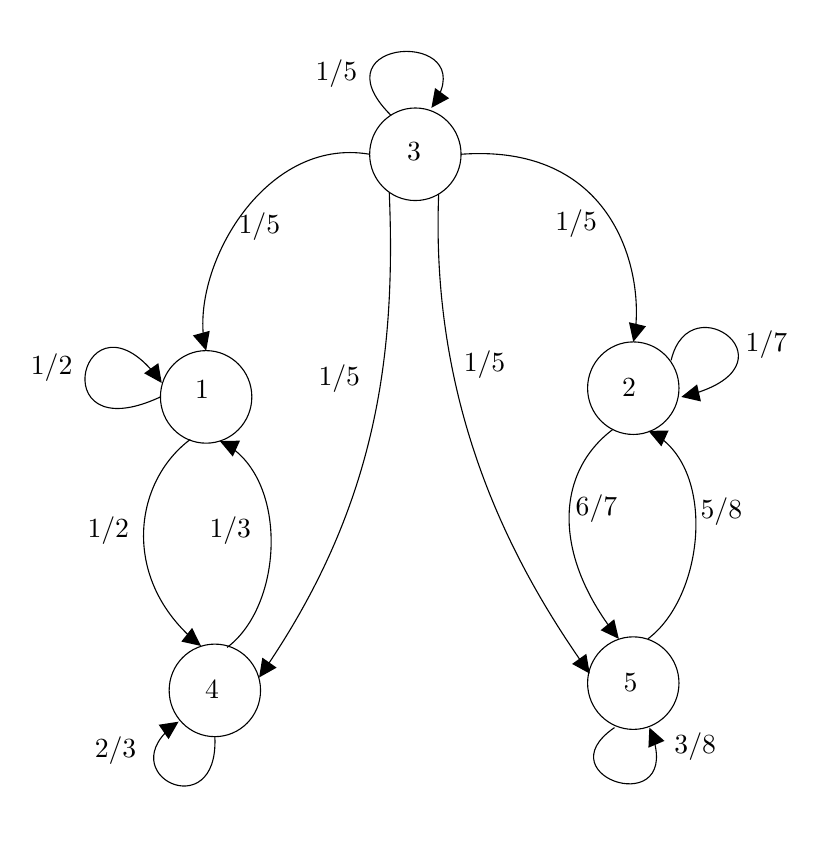
\begin{tikzpicture}[x=0.75pt,y=0.75pt,yscale=-0.7,xscale=0.7]
%uncomment if require: \path (0,714); %set diagram left start at 0, and has height of 714
%Shape: Ellipse [id:dp29836895541013164] 
\draw   (286,156.85) .. controls (286,139.26) and (300.08,125) .. (317.45,125) .. controls (334.82,125) and (348.9,139.26) .. (348.9,156.85) .. controls (348.9,174.44) and (334.82,188.7) .. (317.45,188.7) .. controls (300.08,188.7) and (286,174.44) .. (286,156.85) -- cycle ;
%Shape: Ellipse [id:dp4858180433459096] 
\draw   (142,323.85) .. controls (142,306.26) and (156.08,292) .. (173.45,292) .. controls (190.82,292) and (204.9,306.26) .. (204.9,323.85) .. controls (204.9,341.44) and (190.82,355.7) .. (173.45,355.7) .. controls (156.08,355.7) and (142,341.44) .. (142,323.85) -- cycle ;
%Shape: Ellipse [id:dp10893001214881792] 
\draw   (436,317.85) .. controls (436,300.26) and (450.08,286) .. (467.45,286) .. controls (484.82,286) and (498.9,300.26) .. (498.9,317.85) .. controls (498.9,335.44) and (484.82,349.7) .. (467.45,349.7) .. controls (450.08,349.7) and (436,335.44) .. (436,317.85) -- cycle ;
%Shape: Ellipse [id:dp31584444241771226] 
\draw   (148,525.85) .. controls (148,508.26) and (162.08,494) .. (179.45,494) .. controls (196.82,494) and (210.9,508.26) .. (210.9,525.85) .. controls (210.9,543.44) and (196.82,557.7) .. (179.45,557.7) .. controls (162.08,557.7) and (148,543.44) .. (148,525.85) -- cycle ;
%Shape: Ellipse [id:dp6845584977543557] 
\draw   (436,520.85) .. controls (436,503.26) and (450.08,489) .. (467.45,489) .. controls (484.82,489) and (498.9,503.26) .. (498.9,520.85) .. controls (498.9,538.44) and (484.82,552.7) .. (467.45,552.7) .. controls (450.08,552.7) and (436,538.44) .. (436,520.85) -- cycle ;
%Curve Lines [id:da40673715992947246] 
\draw    (212.24,513.63) .. controls (288.82,402.26) and (304.45,300.14) .. (299.5,183.32) ;
\draw [shift={(209.9,517)}, rotate = 304.9] [fill={rgb, 255:red, 0; green, 0; blue, 0 }  ][line width=0.08]  [draw opacity=0] (12.5,-6.01) -- (0,0) -- (12.5,6.01) -- cycle    ;
%Curve Lines [id:da5133467038577342] 
\draw    (172.69,288.89) .. controls (161.52,237.16) and (212.5,144.11) .. (286,156.85) ;
\draw [shift={(173.45,292)}, rotate = 254.65] [fill={rgb, 255:red, 0; green, 0; blue, 0 }  ][line width=0.08]  [draw opacity=0] (12.5,-6.01) -- (0,0) -- (12.5,6.01) -- cycle    ;
%Curve Lines [id:da008345831811055193] 
\draw    (167.44,493.28) .. controls (114.6,449.49) and (123.1,382.7) .. (162.5,353.15) ;
\draw [shift={(169.9,495.27)}, rotate = 218.21] [fill={rgb, 255:red, 0; green, 0; blue, 0 }  ][line width=0.08]  [draw opacity=0] (12.5,-6.01) -- (0,0) -- (12.5,6.01) -- cycle    ;
%Curve Lines [id:da5634268603548509] 
\draw    (435.25,511.14) .. controls (385.72,441.07) and (327.59,334.04) .. (333.5,184.32) ;
\draw [shift={(437.5,514.32)}, rotate = 234.46] [fill={rgb, 255:red, 0; green, 0; blue, 0 }  ][line width=0.08]  [draw opacity=0] (12.5,-6.01) -- (0,0) -- (12.5,6.01) -- cycle    ;
%Curve Lines [id:da4259073730032066] 
\draw    (187.9,496.27) .. controls (227.3,466.72) and (230.27,378.53) .. (185,355.28) ;
\draw [shift={(182.9,354.27)}, rotate = 384.44] [fill={rgb, 255:red, 0; green, 0; blue, 0 }  ][line width=0.08]  [draw opacity=0] (12.5,-6.01) -- (0,0) -- (12.5,6.01) -- cycle    ;
%Curve Lines [id:da6577514807411684] 
\draw    (468.08,283.01) .. controls (475.64,242.78) and (457.71,148.87) .. (348.9,156.85) ;
\draw [shift={(467.45,286)}, rotate = 283.29] [fill={rgb, 255:red, 0; green, 0; blue, 0 }  ][line width=0.08]  [draw opacity=0] (12.5,-6.01) -- (0,0) -- (12.5,6.01) -- cycle    ;
%Curve Lines [id:da329541870026538] 
\draw    (142,323.85) .. controls (58.35,362.99) and (88.88,241.85) .. (141.3,312.08) ;
\draw [shift={(142.9,314.27)}, rotate = 234.51] [fill={rgb, 255:red, 0; green, 0; blue, 0 }  ][line width=0.08]  [draw opacity=0] (12.5,-6.01) -- (0,0) -- (12.5,6.01) -- cycle    ;
%Curve Lines [id:da3393212160499588] 
\draw    (493.5,298.66) .. controls (506.37,243.94) and (584.91,303.18) .. (503.03,323.29) ;
\draw [shift={(500.5,323.88)}, rotate = 347.23] [fill={rgb, 255:red, 0; green, 0; blue, 0 }  ][line width=0.08]  [draw opacity=0] (12.5,-6.01) -- (0,0) -- (12.5,6.01) -- cycle    ;
%Curve Lines [id:da7968400462935867] 
\draw    (477.5,490.39) .. controls (516.9,460.84) and (525.1,371.56) .. (480,348.28) ;
\draw [shift={(477.9,347.27)}, rotate = 384.44] [fill={rgb, 255:red, 0; green, 0; blue, 0 }  ][line width=0.08]  [draw opacity=0] (12.5,-6.01) -- (0,0) -- (12.5,6.01) -- cycle    ;
%Curve Lines [id:da49532662514959913] 
\draw    (455.47,487.82) .. controls (411.57,431.68) and (414.1,375.7) .. (453.5,346.15) ;
\draw [shift={(457.5,490.39)}, rotate = 231.1] [fill={rgb, 255:red, 0; green, 0; blue, 0 }  ][line width=0.08]  [draw opacity=0] (12.5,-6.01) -- (0,0) -- (12.5,6.01) -- cycle    ;
%Curve Lines [id:da618838807270425] 
\draw    (179.45,557.7) .. controls (182.46,620.43) and (105.86,583.53) .. (152.3,548.96) ;
\draw [shift={(154.5,547.39)}, rotate = 505.54] [fill={rgb, 255:red, 0; green, 0; blue, 0 }  ][line width=0.08]  [draw opacity=0] (12.5,-6.01) -- (0,0) -- (12.5,6.01) -- cycle    ;
%Curve Lines [id:da7726575310463464] 
\draw    (479.68,554.36) .. controls (503.45,616.53) and (404.27,585.93) .. (454.51,551.46) ;
\draw [shift={(478.51,551.46)}, rotate = 67.01] [fill={rgb, 255:red, 0; green, 0; blue, 0 }  ][line width=0.08]  [draw opacity=0] (12.5,-6.01) -- (0,0) -- (12.5,6.01) -- cycle    ;
%Curve Lines [id:da7210031613710599] 
\draw    (330.71,121.65) .. controls (363.66,70.1) and (246.61,75.98) .. (300.51,129.88) ;
\draw [shift={(328.51,124.88)}, rotate = 306.03] [fill={rgb, 255:red, 0; green, 0; blue, 0 }  ][line width=0.08]  [draw opacity=0] (12.5,-6.01) -- (0,0) -- (12.5,6.01) -- cycle    ;
% Text Node
\draw (164,311.21) node [anchor=north west][inner sep=0.75pt]   [align=left] {{\normalsize 1}};
% Text Node
\draw (458,309.21) node [anchor=north west][inner sep=0.75pt]   [align=left] {{\normalsize 2}};
% Text Node
\draw (171,517.21) node [anchor=north west][inner sep=0.75pt]   [align=left] {{\normalsize 4}};
% Text Node
\draw (459,512.21) node [anchor=north west][inner sep=0.75pt]   [align=left] {{\normalsize 5}};
% Text Node
\draw (310,147.21) node [anchor=north west][inner sep=0.75pt]   [align=left] {{\normalsize 3}};
% Text Node
\draw (51,292.21) node [anchor=north west][inner sep=0.75pt]   [align=left] {{\normalsize 1/2}};
% Text Node
\draw (90,404.21) node [anchor=north west][inner sep=0.75pt]   [align=left] {{\normalsize 1/2}};
% Text Node
\draw (543,276.21) node [anchor=north west][inner sep=0.75pt]   [align=left] {{\normalsize 1/7}};
% Text Node
\draw (174,404.21) node [anchor=north west][inner sep=0.75pt]   [align=left] {{\normalsize 1/3}};
% Text Node
\draw (194,195.21) node [anchor=north west][inner sep=0.75pt]   [align=left] {{\normalsize 1/5}};
% Text Node
\draw (426,389.21) node [anchor=north west][inner sep=0.75pt]   [align=left] {{\normalsize 6/7}};
% Text Node
\draw (512,391.21) node [anchor=north west][inner sep=0.75pt]   [align=left] {{\normalsize 5/8}};
% Text Node
\draw (95,556.21) node [anchor=north west][inner sep=0.75pt]   [align=left] {{\normalsize 2/3}};
% Text Node
\draw (494,553.21) node [anchor=north west][inner sep=0.75pt]   [align=left] {{\normalsize 3/8}};
% Text Node
\draw (247,90.21) node [anchor=north west][inner sep=0.75pt]   [align=left] {{\normalsize 1/5}};
% Text Node
\draw (249,300.21) node [anchor=north west][inner sep=0.75pt]   [align=left] {{\normalsize 1/5}};
% Text Node
\draw (349,290.21) node [anchor=north west][inner sep=0.75pt]   [align=left] {{\normalsize 1/5}};
% Text Node
\draw (412,193.21) node [anchor=north west][inner sep=0.75pt]   [align=left] {{\normalsize 1/5}};
\end{tikzpicture}

		
		
		\\  
		&\\
		&\\
		\hline
		\multirow{3}{*}{Checking whether the  } & \\
		& Here,\\states 3 and 1 are in the
		& State 1 is accessible from the state 3.\\same communicating class
	    	& But, State 3 is not accessible from the state 1\\
	    	& \qquad \qquad \qquad i.e.  $3 \rightarrow 1$,  $1 \nrightarrow 3$\\
	    	& \qquad \qquad \qquad$\implies \boxed{3 \nleftrightarrow 1}$\\
	    	&\\ 
	    	&Therefore, 3 and 1 are not in the same communicating class.\\
	   	&\\
	   	\hline
	   \multirow{3}{*}{Checking whether the  } & \\
		& Here,\\states 1 and 4 are in the
		& State 1 is accessible from the state 4.\\same communicating class
	    	& Also, State 4 is accessible from the state 1\\
	    	& \qquad \qquad \qquad i.e.  $3 \rightarrow 1$,  $1 \rightarrow 3$\\
	   	& \qquad \qquad \qquad$\implies \boxed{3 \leftrightarrow 1}$\\
	    	&\\ 
	    	&Therefore, 1 and 4 are in the same communicating class.\\	   	
	   	&\\	   	
	   	\hline
	   	\multirow{3}{*}{Checking whether the  } & \\
		& Here,\\states 4 and 2 are in the
		& State 2 is not accessible from the state 4.\\same communicating class
	    	& Also, State 4 is not accessible from the state 2\\
	    	& \qquad \qquad \qquad i.e.  $4 \nrightarrow 2$,  $2 \nrightarrow 4$\\
	    	\hline
	    	&\\	    	
	   	& \qquad \qquad \qquad$\implies \boxed{4 \nleftrightarrow 2}$\\
	    	&Therefore, 4 and 2 are not in the same communicating class.\\
	   	&\\
	   	\hline
	   	\multirow{3}{*}{Checking whether the  } & \\
		& Here,\\states 2 and 5 are in the
		& State 2 is accessible from the state 5.\\same communicating class
	    	& Also, State 5 is accessible from the state 2\\
	    	& \qquad \qquad \qquad i.e.  $5 \rightarrow 2$,  $2 \rightarrow 5$\\
	   	& \qquad \qquad \qquad$\implies \boxed{2 \leftrightarrow 5}$\\
	    	&\\
	    	&Therefore, 2 and 5 are in the same communicating class.\\
	   	&\\
	   	\hline
	   	\multirow{3}{*}{Conclusion} & \\
	   	&Communication classes are:\\
	   	&\\
	   	& \qquad \qquad \qquad$\boxed{S=\{1,4\}\cup \{3\} \cup \{2,5\}}$\\
	   	&\\
		&Option 2) and 4) are true.\\
	   	&\\
	   	\hline
\caption{Solution}
\label{eq:solutions/2017/dec/105/table1}
    \end{longtable}
%\end{table*}
\twocolumn


%
\item Let $X$ and $Y$ be independent exponential random variables. If $E[X]=1$ and $E[Y]=\frac{1}{2}$ then $\pr{X>2Y|X>Y}$ is
\begin{multicols}{2}
    \begin{enumerate}[label=\arabic*.]
        \item \Large$\frac{1}{2}$ \\
        \item $\frac{1}{3}$
        \item $\frac{2}{3}$ \\
        \item $\frac{3}{4}$
    \end{enumerate}
\end{multicols}
%
\solution
Since $X$ and $Y$ are exponential random variables with means'
\begin{align}
    E[X] = 1 \text{ and } E[Y] = \frac{1}{2}
\end{align}
Marginal PDFs of $X$ and $Y$  are given by
\begin{align}
    f_X(x)= e^{-x} , x>0 \\
    f_Y(y) = 2e^{-2y} , y>0
\end{align}
CDFs for $X$ and $Y$ are
\begin{align}
    F_X(b) &= \int_0^b f_X(x)\,d_x\\
           &= \int_0^b  e^{-x}\,d_x\\
           &= 1-e^{-b}
\end{align}
\begin{align}
    F_Y(b) &= \int_0^b f_Y(y)\,d_y\\
           &= \int_0^b 2e^{-2y}\,d_y\\
           &= \left[-e^{-2y}\right]_0^b\\
           &= 1-e^{-2b}
\end{align}
Now,
\begin{align}
    \pr{X>2Y|X>Y} &= \dfrac{\pr{X>2Y\,,\,X>Y} }{\pr{X>Y}}\\
                  &= \dfrac{\pr{X>2Y}}{\pr{X>Y}} \label{dec2017-59:simul1}
\end{align}
\begin{align}
    \pr{X>Y} &= \pr{Y<X}\\
             &= E[F_Y(X)]\\
             &= \int_0^\infty F_Y(X)\,f_X(x)\,d_x\\
             &= \int_0^\infty (1-e^{-2x})\,e^{-x}d_x\\
             &= \left[\frac{e^{-x}}{-1} - \frac{e^{-3x}}{-3}\right]_0^\infty\\
            &=(0+1)+\frac{1}{3}(0-1) \\
             &= \frac{2}{3} \label{dec2017-59:simul2}
\end{align}
\begin{align}
    \pr{X>2Y} &= \pr{Y<\frac{X}{2}}\\
              &= E[F_Y(X/2)]\\
              &=  \int_0^\infty F_Y(X/2)\,f_X(x)\,d_x\\
              &= \int_{0}^{\infty}(1-e^{-x})\,e^{-x}d_x\\
              &= \left[\frac{e^{-x}}{-1} - \frac{e^{-2x}}{-2}\right]_0^\infty\\
              &= (0+1) + \frac{1}{2}(0-1)\\
              &= \frac{1}{2} \label{dec2017-59:simul3}
\end{align}
Putting \eqref{dec2017-59:simul2} and \eqref{dec2017-59:simul3} in \eqref{dec2017-59:simul1}
\begin{align}
    \pr{X>2Y\,|\,X>Y} &= \frac{1/2}{2/3}\\
                  &= \frac{3}{4}
\end{align}
$\therefore$ Option 4 is the correct answer.


%\item Consider a Markov Chain with state space $\cbrak{0,1,2}$ and transition matrix
%\begin{align}
%P = 
%\begin{blockarray}{c@{\hspace{1pt}}rrr@{\hspace{3pt}}}
%         & 0   & 1   & 2 \\
%        \begin{block}{r@{\hspace{3pt}}@{\hspace{1pt}}
%    (@{\hspace{1pt}}rrr@{\hspace{1pt}}@{\hspace{1pt}})}
%        0 & \frac{1}{2} & \frac{1}{2} & 0  \\
%        1 & 0 &\frac{1}{2}  & \frac{3}{4}  \\
%%
%        2 &  \frac{1}{3} & \frac{1}{3} & \frac{1}{3}  \\
%        \end{block}
%    \end{blockarray}
%\end{align}
%For any two states $i$ and $j$, let $p_{ij}^{(n)}$ denote the $n$-step transition probability of going from $i$ to $j$.  Identify correct statements.
%\begin{enumerate}
%\item $\lim_{n \to \infty} p_{11}^{(n)} = \frac{2}{9}$
%\item $\lim_{n \to \infty} p_{21}^{(n)} = 0$
%\item $\lim_{n \to \infty} p_{32}^{(n)} = \frac{1}{3}$
%\item $\lim_{n \to \infty} p_{13}^{(n)} = \frac{1}{3}$
%\end{enumerate}

\end{enumerate}
